\section{Contexte du stage}

Afin de bien comprendre le sujet de mon stage, il est indispensable d'assimiler 
l'environnement logiciel dans lequel il se positionne, et le problème rencontré 
par les équipes de EPM qui a conduit à la production du programme que j'ai 
écrit.

\subsection{L'intégration continue}

L'intégration continue est un ensemble de pratiques utilisées en génie logiciel.
Elles consistent à vérifier à chaque modification de code source que le résultat
des modifications ne produit pas de régression de l'application en cours de 
développement. L'intégration continue se met en place grâce à deux blocs 
principaux :
\begin{description}
	\item[Source Control Manager (SCM)], qui permet aux développeurs de partager
	le code source d'un projet en le centralisant sur un dépôt. Dans le cadre de
	l'intégration continue, il est indispensable que les programmeurs livrent 
	leur code sur le dépôt très fréquemment. Parmi les SCM les plus connus, on
	trouve Subversion, Git et Mercurial. Thales CST utilise ClearCase.
	\item[Continuous Integration Scheduler/Server], qui intérroge régulièrement 
	le dépôt 
	de source. Si il y a eu modification depuis la dernière compilation, le 
	serveur d'intégration continue lance une nouvelle compilation, les tests 
	associés, et toute autre tâche qui lui a été demandée d'effectuer sur le 
	code en question. Si un problème est détecté, les développeurs sont alertés.
	Exemples de serveur CI: CruiseControl, Hudson, Jenkins, Buildbot, Apache 
	Continuum.
\end{description}

L'intérêt de l'intégration continue est la réactivité qu'elle alloue 
aux développeurs. En effet, avec un processus bien en place, ceux-ci peuvent 
être mis au courant d'une multitude de problèmes provenant du code source, 
au jour le jour, ce qui évite à des bogues de rester dans l'application trop 
longtemps. Du temps et de l'argent est ainsi sauvegardé.

L'intégration continue est donc un outils de contrôle qualité extrêmement 
puissant. De plus, les serveurs prennent généralement en charge des extensions, 
ce qui les rend flexibles et compatibles à de nombreux contextes de 
développement.

\subsection{Qualité du code}

Contrôler la qualité d'un code source consiste à vérifier qu'il vérifie un 
certain nombre de critères. Ces critères peuvent par exemple être: respecter des
conventions syntaxiques, contenir un certain pourcentage de commentaires, 
minimaliser la complexité par fonction ou par classe, être couvert par des tests
unitaires. Des outils d'analyse de code existent afin d'extraire ces 
informations et de les rendre présentables à l'utilisateur. Ces outils sont 
aussi utiles pour les développeurs que pour les chefs de projet, qui peuvent 
ainsi suivre les progrès du projet à l'aide d'une interface attrayante.

Cette technique de qualité peut être couplée avec l'intégration continue de 
manière très intéressante puisque le serveur d'intégration continue peut 
lancer automatiquement les analyses de code voulues et livrer les rapports 
correspondant là où ils sont désirés.

\begin{figure}[htb]
	\centering
	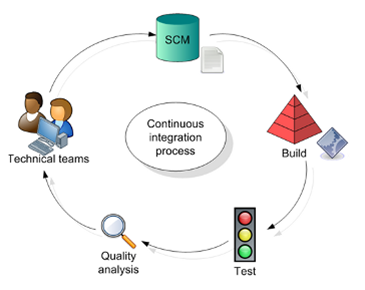
\includegraphics{continuous_integration.png}
	\caption{Le processus d'intégration continue couplé à l'analyse qualité}
\end{figure}

\subsection{ThalesControl}
\label{ThalesControl}

Afin d'améliorer la compétitivité des entités Thales, EPM développe au sein 
de l'équipe Code Building une 
solution d'intégration continue clé en main, appelée ThalesControl. Elle couple 
un serveur d'intégration continue, Hudson, et un aggrégateur de métriques de 
qualité, Sonar. Ces logiciels ne sont pas développés par Thales, et sont 
libres et gratuits. Le travail de Thales CST sur ThalesControl consiste à assurer 
une compatiblité parfaite entre les logiciels au fur et à mesure de leurs
mises à jour respectives. Le second objectif de ThalesControl est de s'adapter
à toutes les entités, qui utilisent des outils de développement très variés. 
Thales CST ajoute donc à Hudson et Sonar une multitude d'extensions pour l'un et
pour l'autre, afin qu'ils prennent en charge différents SCM, moteur de 
production (Make, Gradle, Maven, Ant...), plate-formes de test (xUnit), langages
de programmation, ou autres composants de la chaîne de construction de 
l'application cible. Chaque extension à sa propre progression. Certaines sont 
développées par la communauté libre, d'autres par Thales CST, d'autres encore 
par des entités Thales différentes. L'équipe ThalesControl doit donc jongler 
avec toutes ces briques logiciels (environ 80) dont les versions changent 
sans cesse, regrouper un ensemble qui fonctionne, et livrer le résultat.

ThalesControl est hautement personnalisable : il est possible d'installer ou non
un composant et de choisir la version de chaque composant.

\begin{figure}[htb]
	\centering
	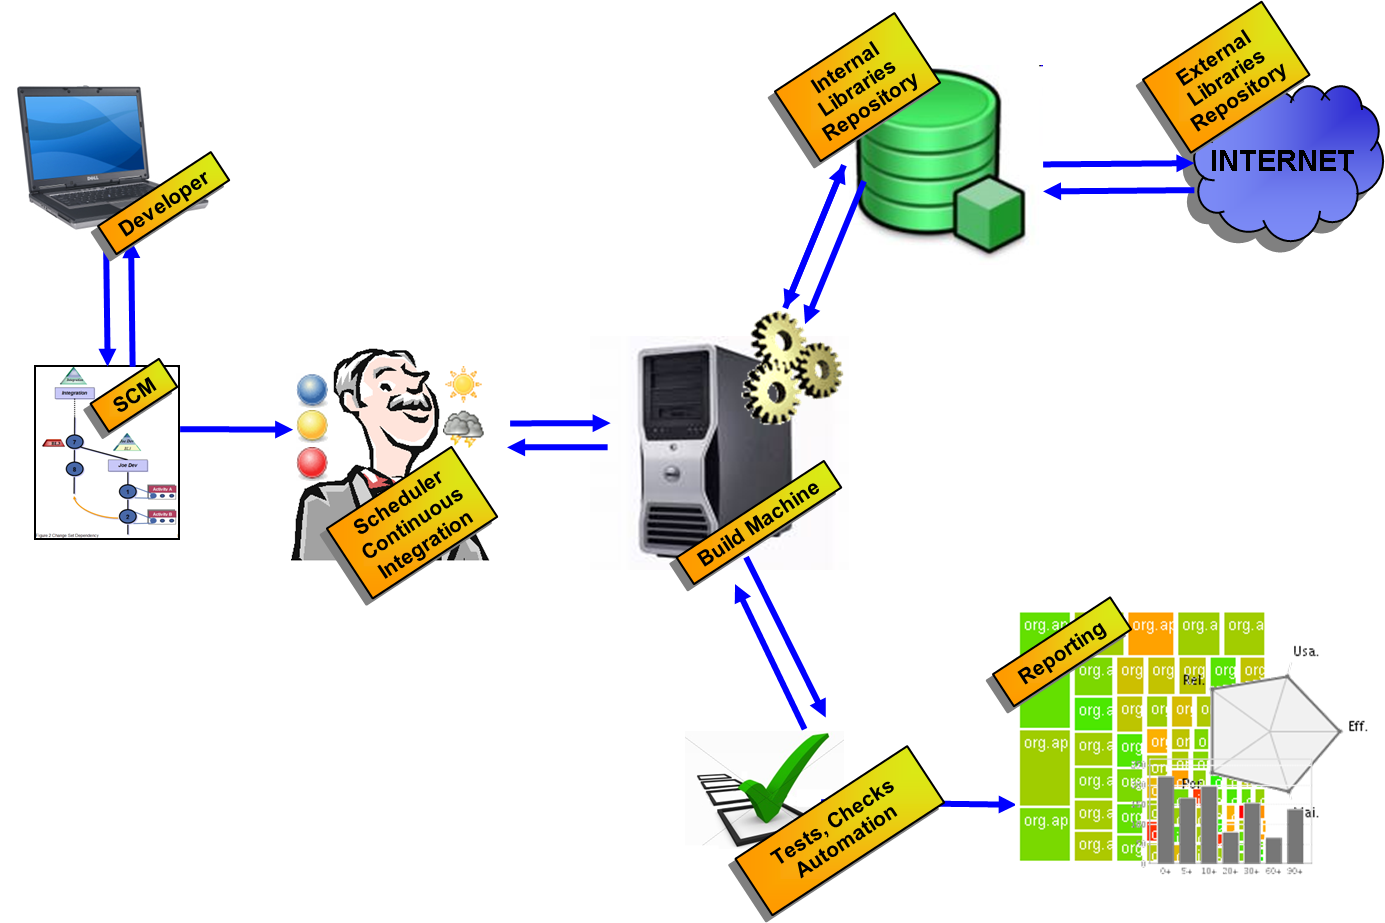
\includegraphics[scale=0.5]{continuous_integration_with_thales_control.png}
	\caption{L'intégration continue avec ThalesControl}
\end{figure}

Additionnellement, ThalesControl est fourni avec un installateur qui installe et
configure tous les composants selon les désirs de l'utilisateur. Ces désirs 
doivent être spécifiés dans un fichier de configuration écrit à l'avance.

On peut remarquer ici que l'équipe ThalesControl utilise de nombreux programmes libres. 
J'aimerais préciser que l'entreprise ne se contente pas d'utiliser ces 
logiciels, mais participe activement à leur développement, notamment par le 
biais d'extensions, que Thales met généralement sous licence libre 
et à disposition de la communauté. Cette philosophie, défendue par Jérôme Vacher,
est justifiée par le fait que Thales CST est un centre de coût pour Thales, et
n'a pas vocation à générer de profits.  Elle ne peut donc que tirer avantage 
de la communauté open-source, qui présente une source d'idées et de testeurs, 
ainsi que, parfois, de développeurs. C'est donc un moyen de réduire les coûts.

\subsection{La problématique Hudson/Jenkins}
\label{Hudson_Jenkins}

La communauté autour de Hudson a vu d'un mauvais {\oe}il le rachat de Sun 
Microsystems, détenteur des droits d'exploitation du nom Hudson et développeur 
originel du projet, par Oracle en 2010. Après des négociations non-abouties 
entre la dite communauté et Oracle, la première a décidé de créer une nouvelle 
branche du projet n'étant pas sous le contrôle d'Oracle. Le nouveau logiciel 
ainsi né a été nommé Jenkins. Oracle a de son côté conservé Hudson, puis l'a 
donné à la Fondation Eclipse, organisation majeure du monde du logiciel libre. 
Les deux logiciels cohabitent à présent, et sont tout deux activement développés.

Ces évènements impactent évidemment ThalesControl puisque l'équipe doit choisir 
quelle branche suivre. Durant mon stage, aucune décision finale n'a été prise.
La prochaine version de ThalesControl devait être livrée avec la version de 
Hudson distribuée juste avant la séparation, vieille de plusieurs mois.

Le problème est que la plupart des extensions avait déjà fait leur choix et 
nombre d'entre elles étaient déjà disponibles pour la dernière version de 
Jenkins. L'équipe de ThalesControl se voyait donc dans l'obligation, pour se 
maintenir à jour et pour répondre aux demandes de ses utilisateurs, d'essayer 
de fournir des extensions Jenkins avec Hudson. Tester à la main chacune des 
extensions et éventuellement les modifier pour les rendre compatibles est un 
travail trop important.

Le besoin d'un outil de test de compatibilité automatique entre serveur 
d'intégration et extensions est alors devenu critique.

\subsection{La problématique Sonar}
\label{ProbSonar}

Sonar est mis à jour très régulièrement. Une mise à jour majeure voit le jour 
environ tous les 3 mois. Ces mises à jour cassent souvent l'interface de 
programmation des extensions pour Sonar. Cela veut dire qu'à chaque nouvelle 
version, les développeurs des extensions doivent modifier leur code. Thales 
CST a créé une extension pour Sonar 2.0, mais n'a pas les 
ressources pour la maintenir. Ainsi pendant plus d'un an ThalesControl a été 
livré avec Sonar 2.0 alors que pendant ce laps de temps 7 versions de Sonar sont 
sorties.

Sous la pression des utilisateurs, Thales CST a du allouer du temps et des 
ressources à la migration de Sonar 2.0 à Sonar 2.8 (puis 2.9 et 2.10, sorties 
rapidement après). La problèmatique principale a été de trouver un moyen 
d'implémenter les mêmes fonctionnalités que l'extension pour Sonar 2.0, 
mais d'une manière requierant moins de maintenance à chaque nouvelle version de 
Sonar.

Durant ce processus, l'équipe ThalesControl a examiné plusieurs solutions et a 
pour cela du étudier Sonar de plus près. En particulier, l'organisation de la 
base données de Sonar ainsi que les modifications qui lui sont apportées entre 
chaque nouvelle version ont été observées. Le besoin s'est alors fait sentir 
de posséder un outils capable de comparer des bases de donneés et de fournir 
un résultat lisible et exploitable.

\subsection{La solution TCtest}
\label{TCtest}

\subsubsection{Objectif}

Afin de délester le personnel des tâches répétitives de test d'intégration 
entre les composants de ThalesControl, il a été décidé de développer un outil 
automatisant au mieux ces tâches. Cet outil a été nommé TCtest. Un premier 
stagiaire, Francis Ngougo, 
a programmé un premier jet d'un tel programme pendant 6 mois fin 2010.
Il est important de préciser qu'un des objectifs 
de TCtest est d'être tout-terrain. C'est-à-dire qu'il doit être capable de :
\begin{itemize}
	\item{travailler avec n'importe quelle installation de ThalesControl, sachant que 
	celui-ci est constitué d'environ 80 composants dont la fréquence de renouvellement 
	est très rapide;}
	\item{travailler avec de multiples installations de ThalesControl en même 
	temps;}
	\item{permettre à l'utilisateur de créer de nouveaux jeux de tests sans 
	toucher au code source.}
\end{itemize}

\subsubsection{Vocabulaire}
\label{Voc}

\begin{description}
	\item[Service] Brique logiciel compilée en une librairie (un fichier JAR 
	dans le cas présent). Les services sont découverts et chargés dynamiquement 
	par TCtest. Les services effectuent généralement des tâches très simples.
	\item[Workflow] Synonymes de test, c'est-à-dire une séquence d'actions qui 
	produit généralement un résultat booléen (réussi ou non). Les workflows 
	sont définis par l'utilisateur dans des fichiers XML. Les actions en 
	questions sont effectuées par des services. Un workflow est donc une 
	séquence de services, avec éventuellement des paramètres pour chaque 
	service.
	\item[Instance de ThalesControl] Ensemble de composants (chacun associé
	à une version) formant un produit ThalesControl.
\end{description}

\subsubsection{Principe}

Je présenterai seulement succintement le logiciel
dans cette partie, et détaillerai au besoin dans la partie Réalisation. TCtest 
fonctionne suivant 4 étapes :
\begin{description}
	\item[Initialisation]{
	TCtest lit des fichiers de configuration écrit par l'utilisateur. Ces 
	fichiers décrivent premièrement l'environnement (dans quel dossier chercher 
	les tests disponibles, dans quel dossier installer ThalesControl...) et 
	deuxièmement quels tests (aussi appelés workflows) lancer, et sur quelles 
	instances de ThalesControl. La configuration fait référence à ces éléments 
	par le nom du dossier dans lequel trouver leur définition, sachant que ces
	définitions sont écrites en XML.}
	\item[Installation]{
	TCtest installe toutes les instances de ThalesControl qui lui sont demandées de 
	tester, grâce à l'installateur.}
	\item[Lancement]{
	TCtest lance les composants de ThalesControl qui requièrement un tel lancement 
	(Tomcat, Hudson, Sonar...).}
	\item[Test]{
	TCtest lit les définitions (fichiers XML) des tests qui lui sont demandés 
	d'effectuer puis exécute les tests. L'exécution comprend la lecture d'un fichier
	de workflow, l'instanciation puis l'exécution des services mentionnés dans ce 
	workflow.}
\end{description}

Je conseille fortement au lecteur intéressé de lire le manuel utilisateur (en 
Anglais) de TCtest 5.0, que j'ai écrit lors de mon stage. Le manuel se trouve en
annexe de ce rapport.

\subsubsection{Parallélisation}
\label{Parallel}

TCtest 1.0 est implémenté sous forme de pipeline. Les étapes d'installation, de 
lancement et de test sont chacune traitées par un thread différent. Les 3 threads 
prennent leurs entrées et mettent leurs sorties dans des files. Cela signifie 
qu'il est possible de tester une première instance pendant qu'une seconde 
s'installe. TCtest étant destiné à travailler sur de grandes batteries de tests,
ce processus a été mis en place pour gagner du temps.

\subsubsection{Modularité}

TCtest se décompose en plusieurs modules :
\begin{description}
	\item[Le lanceur]{C'est l'application principale, que l'on configure et que
	l'on lance pour effectuer les tests}
	\item[L'API]{C'est l'ensemble des interfaces et classes fournies aux 
	développeurs tiers afin qu'ils puissent étendre les fonctionnalités de 
	TCtest.}
	\item[Les services]{Voir \ref{Voc}.}
\end{description}
